\section{Data normalization in DNNs and CNNs}

\subsection{Normalization for input data of DNNs}
Consider that we have the all training data as
\begin{equation}\label{eq:trainingdata}
(X,Y) := \{(x_i, y_i)\}_{i=1}^N,
\end{equation}
for $x_i \in \mathbb{R}^d$ and $y_i \in \mathbb{R}^k$.

Before we input every data into a DNN model, we will apply the following normalization
for all data $x_i$ for each component.
Let denote
\begin{equation}\label{key}
[x_i]_j \longleftrightarrow \text{ the j-th component of data } x_i.
\end{equation}
Then we have following formula of for all $j = 1, 2, \cdots, d$
\begin{equation}\label{key}
[\tilde x_i]_j  = \frac{[x_i]_j - [\mu_X]_j }{\sqrt{[\sigma_X]_j}},
\end{equation}
where 
\begin{equation}\label{key}
[\mu_X]_j =\mathbb{E}_{x \sim X}[[x]_j] = \frac{1}{N}\sum_{i=1}^N [x_i]_j, 
\quad  [\sigma_X]_j = \mathbb{V}_{x\sim X}[[x]_j] = \frac{1}{N} \sum_{i=1}^N ( [x_i]_j - [\mu_X]_j)^2.
\end{equation}
Here $x \sim X$ means that $x$ is a discrete random variable on $X$
with probability
\begin{equation}\label{key}
\mathbb P( x = x_i ) = \frac{1}{N},
\end{equation}
for any $x_i \in X$.

For simplicity, we rewrite the element-wise definition above as the following
compact form
\begin{equation}\label{eq:normlizationData}
\tilde x_i = \frac{x_i - \mu_X }{\sqrt{\sigma_X}},
\end{equation}
where
\begin{equation}\label{key}
x_i , \tilde x_i , \mu_X, \sigma_X \in \mathbb{R}^d,
\end{equation}
defined as before and all operations in \eqref{eq:normlizationData} are element-wise.


Here we note that, by normalizing the data set, we have the next properties 
for new data $\tilde x \in \tilde X$ with component $j = 1,2,\cdots,d$,
\begin{equation}\label{key}
\mathbb{E}_{\tilde X}[[\tilde x]_j] = \frac{1}{N} \sum_{i=1}^N [\tilde x_i]_j = 0,
%\begin{pmatrix}
%0\\0\\\vdots\\0 
%\end{pmatrix} \in \mathbb{R}^d,
\end{equation}
and 
\begin{equation}\label{key}
\mathbb{V}_{\tilde X}[[\tilde x]_j] = \frac{1}{N} \sum_{i=1}^N ([\tilde x_i]_j - \mathbb{E}_{\tilde X}[[\tilde x]_j] )^2 = 1.
%\begin{pmatrix}
%1\\1\\\vdots\\1 
%\end{pmatrix} \in \mathbb{R}^d.
\end{equation}

Finally, we will have a ``new'' data set 
\begin{equation}\label{key}
\tilde X = \{\tilde x_1, \tilde x_2, \cdots, \tilde x_N \},
\end{equation}
with unchanged label set $Y$. For the next sections, without special notices, we use $X$ data set
as the normalized one as default. 


\subsection{Data normalization for images in CNNs}
For images, consider we have a color image data set $(X,Y) := \{(x_i, y_i)\}_{i=1}^N$ where
\begin{equation}\label{key}
x_i \in \mathbb{R}^{3 \times m\times n}.
\end{equation}
We further denote these the $(s,t)$ pixel value for data $x_i$ at channel $j$ as:
\begin{equation}\label{key}
[x_i]_{j;st} \longleftrightarrow (s,t) \text{ pixel value for } x_i \text{ at channel } j,
\end{equation}
where $1\le i \le N, 1\le j\le 3, 1\le s \le m$, and  $1\le j\le n$.

Then, the normalization for $x_i$ is defined by
\begin{equation}\label{key}
[\tilde x_i]_{{j;st}} = \frac{[x_i]_{{j;st}} - [\mu_X]_j }{\sqrt{[\sigma_X]_j}},
\end{equation}
where %$\bm 1 \in \mathbb{R}^{m\times n}$ with all elements equal to $1$ and
\begin{equation}\label{key}
[x_i]_{{j;st}}, [\tilde x_i]_{{j;st}}, [\mu_X]_j, [\sigma_X]_j \in \mathbb{R}.
\end{equation}
Here 
\begin{equation}\label{key}
[\mu_X]_j = \frac{1}{m\times n\times N} \sum_{ 1 \le i \le N} \sum_{1\le s \le m, 1 \le t \le n} [x_i]_{j;st}.
\end{equation}
and 
\begin{equation}\label{key}
[\sigma_X]_j = \frac{1}{ N \times m\times n} \sum_{ 1 \le i \le N} \sum_{1\le s \le m, 1 \le t \le n} ([x_i]_{j;st} -[\mu_X]_j )^2.
\end{equation}
In batch normalization, we confirmed with Lian by both numerical test and code checking that BN also use the above 
formula to compute the variance in CNN for each channel.


Another way to compute the variance over each channel is to compute the standard deviation on each channel for every data,
and then average them in the data direction.
\begin{equation}\label{key}
\sqrt{[\tilde \sigma_X]_j} = \frac{1}{ N} \sum_{ 1 \le i \le N}  \left( \frac{1}{m\times n}\sum_{1\le s \le m, 1 \le t \le n} ([x_i]_{j;st} - [\mu_i]_j )^2 \right)^{\frac{1}{2}},
\end{equation}
where
\begin{equation}\label{key}
[\mu_i]_j  = \frac{1}{m\times n} \sum_{1\le s \le m, 1 \le t \le n} [x_i]_{j;st}.
\end{equation}

\subsection{Comparison of $\sqrt{[\sigma_X]_j}$ and  $\sqrt{[\tilde \sigma_X]_j}$ on CIFAR10.}

They share the same $\mu_X$ as
\begin{equation}\label{key}
\mu_X = \begin{pmatrix}
0.49140105 & 0.48215663 & 0.44653168
\end{pmatrix}.
\end{equation}
But they had different standard deviation estimates:
\begin{equation}
\begin{aligned}
\sqrt{[\sigma_X]_j} &= \begin{pmatrix}
0.24703284 & 0.24348499 & 0.26158834
\end{pmatrix} \\
%\sqrt{[\bar \sigma_X]_j} &= \begin{pmatrix}
%0.12835675 & 0.12578563 & 0.1533168
%\end{pmatrix} \\
\sqrt{[\tilde \sigma_X]_j} &= \begin{pmatrix}
0.20220193 & 0.19931635 & 0.20086373
\end{pmatrix} 
\end{aligned}
\end{equation}

\section{Initialization for deep neural networks}

\subsection{Xavier's Initialization}
The goal of Xavier initialization~\cite{glorot2010understanding} is to initialize the deep neural network to avoid gradient vanishing or blowup when the input is white noise.

Let us denote the DNN models as:
\begin{equation}
\begin{cases}
f^1(x) &= W^1 x + b^1 \\
f^{\ell}(x) &= W^\ell \sigma(f^{\ell-1}(x)) + b^\ell \quad \ell = 2:L \\
f(x) &= f^{L} \\
\end{cases},
\end{equation}
with $x \in \mathbb{R}^{n_0}$ and $f^{\ell} \in \mathbb{R}^{n_\ell}$. More precisely, we have
\begin{equation}\label{key}
W^\ell \in \mathbb{R}^{n_{\ell} \times n_{\ell-1}}.
\end{equation}

The basic assumptions that we make are:
\begin{itemize}
	%% \item The input $x$ is a mean $0$ random variable with identity covariance, i.e. $\mathbb{E}(x) = 0$, $\mathbb{E}(x_ix_j) = 0$ if $i\neq j$, and $\mathbb{E}(x_i^2) = 1$
	% \item \blue{The input $x$ is a mean $0$ random vector with the same variance for each component, i.e. $\mathbb{E}[[x]_i] = 0$ and $\mathbb{E}[[x]_i^2] (\mathbb{V} [[x]_i]) =$ $\mathbb{E}[[x]_j^2] (\mathbb{V}[[x]_j])$. }
	% (Here we notice that, after data normalization as discussed before this assumption holds directly.)
	\item The initial weights $W^\ell_{ij}$ are i.i.d symmetric random variables with mean $0$, namely the 
	probability density function of $W^\ell_{ij}$ is even.
	\item The initial bias $b^\ell = 0$.
\end{itemize}


Now we choose the variance of the initial weights to ensure that the features $f^L$ and gradients don't blow up or vanish. To this end we have the following lemma.

\begin{lemma}\label{lemm:init}
	Under the previous assumptions $f^\ell_i$  is a symmetric random variable with $\mathbb{E}[f^\ell] = 0$.
	Moreover, we have the following identity
	\begin{equation}\label{eq:FWini}
	\mathbb{E}[(f^{\ell}_i)^2] = \sum_{k}\mathbb{E}[(W^\ell_{ik})^2]\mathbb{E}[\sigma(f^{\ell-1}_k)^2].
	\end{equation}
	% \begin{equation}\label{key}
	%  \mathbb V [f^{L}_i] =  \left(\Pi_{\ell=1}^{L} n_{\ell-1} {\rm Var} [W^\ell_{st}] \right)\mathbb V [x_j].
	% \end{equation}
\end{lemma}
%Note that here we don't have that $f^\ell_i$ and $f^\ell_j$ are actually independent, just that they are `linearly' independent.



Now, if $\sigma  = id$, we can prove by induction from $\ell = 1$ that
	\begin{equation}\label{key}
	\mathbb V [f^{L}_i] =  \left(\Pi_{\ell=2}^{L} n_{\ell-1} {\rm Var} [W^\ell_{st}] \right) \left(\mathbb{V}[W^1_{st}]\sum_{k}\mathbb{E}[( [x]_k)^2] \right).
	\end{equation}
We make this assumption that $\sigma  = id$, which is pretty reasonably since most activation functions in use at the time (such as the hyperbolic tangent) were close to the identity near $0$.

Now, if we set 
\begin{equation}\label{key}
\mathbb{V}[W^\ell_{ik}] = \frac{1}{n_{\ell-1}}, \quad \forall \ell \ge 2,
\end{equation}
we will obtain
\begin{equation}
\mathbb V [f^{L}_i] = \mathbb V [f^{L-1}_j] = \cdots =  \mathbb V [f^{1}_k] = \mathbb{V}[W^1_{st}]\sum_{k}\mathbb{E}[( [x]_k)^2].
\end{equation}

Thus, in pure DNN models, it is enough to just control $\sum_{k}\mathbb{E}[( [x]_k)^2]$.

A similar analysis of the propagation of the gradient ($\frac{\partial L(\theta)}{\partial f^\ell}$) suggests that we set 
\begin{equation}\label{key}
\mathbb{V}[W^\ell_{ik}] = \frac{1}{n_{\ell}}.
\end{equation}


Thus, the {\bf Xavier's initialization} suggests to initialize $W^\ell_{ik}$ with variance as:
\begin{itemize}
	\item To control $\mathbb V [f^{\ell}_i] $:
	\begin{equation}\label{key}
	{\rm Var}[W^\ell_{ik}] = \frac{1}{n_{\ell-1}}.
	\end{equation}
	\item To control $\mathbb{V}[\frac{\partial L(\theta)}{\partial f_i^\ell}]$:
	\begin{equation}\label{key}
	{\rm Var}[W^\ell_{ik}] = \frac{1}{n_{\ell}}.
	\end{equation}
	\item Trade-off to control $\mathbb{V} [\frac{\partial L(\theta)}{\partial W_{ik}^\ell}]$: 
	\begin{equation}\label{key}
	{\rm Var}[W^\ell_{ik}] = \frac{2}{n_{\ell-1} + n_\ell}.
	\end{equation}
\end{itemize}

Here we note that, this analysis works for all symmetric type distribution around zero, 
but we often just choose uniform distribution $\mathcal U(-a,a)$ and normal distribution $\mathcal N(0,s^2)$.
Thus, the final version of Xavier's initialization takes the trade-off type as
\begin{equation}
W^{\ell}_{ik} \sim \mathcal{U}(-\sqrt{\frac{6}{n_\ell+n_{\ell-1}}}, \sqrt{\frac{6}{n_\ell+n_{\ell-1}}}),
\end{equation}
or
\begin{equation}
W^{\ell}_{ik} \sim \mathcal{N}(0,  {\frac{2}{n_\ell+n_{\ell-1}}}).
\end{equation}


%\subsection{Variance analysis in backward propagation phase}
%See the separate file in {``6DL/HandWrittenNotes/InitBackward.pdf''}
%\includepdf[pages=-,pagecommand={}]{HandWrittenNotes/InitBackward.pdf}
%\includepdf[pages=-,pagecommand={}]{497/handwritten_notes/MultidimensionalVariance.pdf}


\subsection{Kaiming's initialization}
In~\cite{he2015delving}, Kaiming He and others extended this analysis to get an \textit{exact} result when the activation function is the {\bf ReLU}.

We first have the following lemma for symmetric distribution.
\begin{lemma}
	If $X_i \in \mathbb{R}$ for $i=1:n$ are i.i.d with symmetric probability density function $p(x)$, i.e. $p(x)$ is even.
	Then for any nonzero random vector $Y = (Y_1, Y_2, \cdots, Y_n) \in \mathbb{R}^n$ which is independent with $X_i$, 
	the following random variable
	\begin{equation}\label{key}
	Z = \sum_{i=1}^n X_i Y_i,
	\end{equation} 
	is also symmetric.
\end{lemma}


Then state the following result for ReLU function and random variable with 
symmetric distribution around $0$.
\begin{lemma}
	If $X$ is a random variable on $\mathbb{R}$ with symmetric probability density $p(x)$ around zero, i.e., 
	\begin{equation}\label{key}
	p(x) = p(-x).
	\end{equation}
	Then we have $\mathbb{E} X = 0$ and 
	\begin{equation}\label{key}
	\mathbb{E}[[{\rm ReLU}(X)]^2] = \frac{1}{2}{\rm Var}[X].
	\end{equation}
\end{lemma}


Based on the previous Lemma~\ref{lemm:init}, we know that $f^{\ell-1}_k$ is a symmetric distribution around $0$.
The most important observation in Kaiming's paper~\cite{he2015delving} is that:
\begin{equation}\label{key}
\mathbb{V}[ f^\ell_i ] = n_{\ell-1}  \mathbb{V}[W^\ell_{ij}] {\mathbb{E}[[\sigma(f^{\ell-1}_j)]^2]} = n_{\ell-1} \mathbb{V}[W^\ell_{ik}] {\frac{1}{2} \mathbb{V}[f^{\ell-1}_k]},
\end{equation}
{if $\sigma = {\rm ReLU}$}.
Thus, Kaiming's initialization suggests to take:
\begin{equation}\label{key}
\mathbb{V}[W^\ell_{ik}] = \frac{2}{n_{\ell-1}}, \quad \forall \ell \ge 2.
\end{equation}

For the first layer $\ell=1$, by definition
\begin{equation}\label{key}
f^1 = W^1 x + b^1,
\end{equation}
there is no ReLU, thus it should be $\mathbb{V}[W^1_{ik}] = \frac{1}{d}$. 
For simplicity, they still use $\mathbb{V}[W^1_{ik}] = \frac{2}{d}$ in the paper~\cite{he2015delving}.
Similarly, an analysis of the propagation of the gradient suggests that we set 
$\mathbb{V}[W^\ell_{ik}] = \frac{2}{n_{\ell}}$.
However, in paper~\cite{he2015delving} authors did not suggest to take the trade-off version, they just chose 
\begin{equation}\label{key}
\mathbb{V}[W^\ell_{ik}] = \frac{2}{n_{\ell-1}},
\end{equation} as default.

Thus, the final version of Kaiming's initialization takes the forward type as
\begin{equation}
W^{\ell}_{ik} \sim \mathcal{U}(-\sqrt{\frac{6}{n_{\ell-1}}}, \sqrt{\frac{6}{n_{\ell-1}}}),
\end{equation}
or
\begin{equation}
W^{\ell}_{ik} \sim \mathcal{N}(0,  {\frac{2}{n_{\ell-1}}}).
\end{equation}

%And another difference is that Xavier use the uniform distribution but He use the Gaussian distribution. 
%More precisely, 
%However, in Pytorch implementation, the uniform distribution is also applied.



\subsection{Initialization in CNN models and experiments}
For CNN models, following the analysis above we have the next iterative scheme in CNNs
\begin{equation}\label{key}
f^{\ell,i} = K^{\ell,i} \ast \sigma (f^{\ell,i-1}),
\end{equation}
where $f^{\ell,i-1} \in \mathbb{R}^{c_\ell\times n_\ell \times m_\ell }$, $f^{\ell,i} \in \mathbb{R}^{h_\ell\times n_\ell \times m_\ell}$ and $K \in \mathbb{R}^{(2k+1) \times (2k+1) \times h_\ell \times c_\ell}$.
Thus we have
\begin{equation}\label{key}
[f^{\ell,i}]_{h;p,q} = \sum_{c=1}^{c_\ell}\sum_{s,t=-k}^k K^{\ell,i}_{h,c;s,t} \ast \sigma ([f^{\ell,i-1}]_{c;p+s,q+t}).
\end{equation}
Take variance on both sides, we will get
\begin{equation}\label{key}
\mathbb{V} [[f^{\ell,i}]_{h;p,q}] = c_\ell (2k+1)^2 \mathbb{V}[K^{\ell,i}_{h,o;s,t}] \mathbb{E}[([f^{\ell,i-1}]_{o;p+s,q+t})^2],
\end{equation}
thus we have the following initialization strategies:
\begin{description}
	\item[Xavier's initialization] 
	\begin{equation}\label{key}
	\mathbb{V}[K^{\ell,i}_{h,o;s,t}] = \frac{2}{ (c_\ell + h_\ell) (2k+1)^2}.
	\end{equation}
	\item[Kaiming's initialization]
	\begin{equation}\label{key}
	\mathbb{V}[K^{\ell,i}_{h,o;s,t}] = \frac{2}{c_\ell (2k+1)^2}.
	\end{equation}
\end{description}

Here we can take this Kaiming's initialization as:
\begin{itemize}
	\item Double the Xavier's choice, and get
	\begin{equation}\label{key}
	\mathbb{V}[K^{\ell,i}_{h,o;s,t}] = \frac{4}{(c_\ell + h_\ell )(2k+1)^2}.
	\end{equation}
	\item Then pick $c_\ell$ or $h_\ell$ for final result
	\begin{equation}\label{key}
	\mathbb{V}[K^{\ell,i}_{h,o;s,t}] = \frac{4}{(c_\ell + h_\ell )(2k+1)^2} = \frac{2}{c_\ell (2k+1)^2}.
	\end{equation}
\end{itemize}

And they have the both uniform and normal distribution type.
\begin{figure}[H]
	\begin{center}
		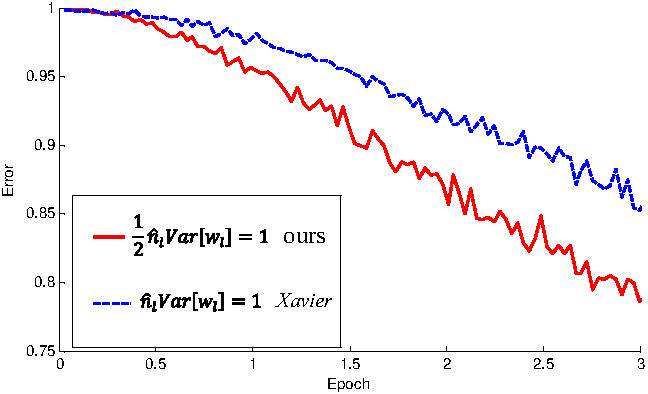
\includegraphics[width=0.45\linewidth]{converge_22layers}
	\end{center}
	\caption{The convergence of a \textbf{22-layer} large model. The x-axis is the number of training epochs. The y-axis is the top-1 error of 3,000 random val samples, evaluated on the center crop. Use ReLU as the activation for both cases. Both Kaiming's initialization (red) and ``\emph{Xavier's}'' (blue) \cite{glorot2010understanding} lead to convergence, but Kaiming's initialization starts reducing error earlier.}
	\label{fig:converge_22layers}
	%\end{figure}
	%\begin{figure}[t]
	\begin{center}
		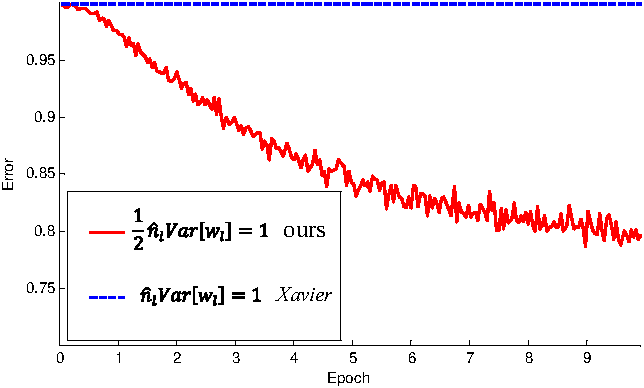
\includegraphics[width=0.45\linewidth]{converge_30layers}
	\end{center}
	\caption{The convergence of a \textbf{30-layer} small model (see the main text). Use ReLU as the activation for both cases. Kaiming's initialization (red) is able to make it converge. But ``\emph{Xavier's}'' (blue) \cite{glorot2010understanding} completely stalls - It is also verified that that its gradients are all diminishing. It does not converge even given more epochs.}
	\label{fig:converge_30layers}
\end{figure}

Given a 22-layer model, in cifar10 the convergence with Kaiming's initialization is faster than Xavier's, 
but both of them are able to converge and the validation accuracies with two different initialization 
are about the same(error is 33.82,33.90).

With extremely deep model with up to 30 layers, 
Kaiming's initialization is able to make the model convergence. On the contrary, Xavier's method completely stalls the learning.


\section{Batch Normalization in DNN and CNN}
\subsection{Recall the original DNN model}
Consider the classical (fully connected)  artificial deep neural network (DNN) $f^L$,
\begin{equation}\label{nn}
\begin{cases}
f^1&= \theta^1 (x) := W^1 x+b^1,\\
f^\ell &= \theta^{\ell} \circ \sigma (f^{\ell-1}) :=W^\ell  \sigma (f^{\ell-1}) +b^\ell,\ \ell=2,...,L.
\end{cases}
\end{equation}
where $x\in\mathbb{R}^n$ is the input vector, $\sigma$ is a non-linear function (activation).  


\subsection{``Real'' Batch Normalization and ``new'' model}
\paragraph{Definition of BN operation based on the batch}
Following the idea in normalization, we consider that we have the all
training data as
\begin{equation}\label{eq:trainingdata}
(X,Y) := \{x_i, y_i\}_{i=1}^N.
\end{equation}

Since the normalization is applied to
each activation independently, let us focus on a particular activation $ [f^\ell]_k$ and omit $k$ as $f^\ell$ for clarity. 
We have $N$ values of this activation
in the batch,
$$ X=\{x_1, \cdots, x_N\}.$$ 
Let the normalized values be
$\hat f^\ell$, and their linear transformations be $\tilde f^\ell$. 
\begin{equation}\label{def:BNeq}
\begin{aligned}
\mu^\ell_{ X} & \leftarrow \mathbb{E}_{x \sim X} [f^\ell(x)] =  \frac{1}{N}\sum_{i=1}^N f^\ell(x_i) & \text{ batch mean}& \\
\sigma^\ell_{ X} & \leftarrow \mathbb{E}_{x \sim X}  \left[(f^\ell(x)-\mathbb{E}_{x \sim X}[ f^\ell(x)])^2 \right] = \frac{1}{N}\sum_{i=1}^N (f^\ell(x_i)-\mu_{ X})^2 &  \text{ batch variance}&\\
\hat f^\ell (x) & \leftarrow \frac{f^\ell(x)-\mu^\ell_{ X}}{\sqrt{\sigma^\ell_{ X}+\epsilon}}   &\text{ normalize}&\\
\tilde f^\ell(x)  & \leftarrow \gamma^\ell \hat f^\ell (x) + \beta^\ell 
&\text{ scale and shift}&
\end{aligned}
\end{equation}
Here we note that all these operations in the previous equation are defined by element-wise.
Then at last, we define the BN operation based on the batch set as
\begin{equation}\label{eq:BNop}
{\rm BN}_{X}({f^\ell(x)}) = \tilde f^\ell(x) := \gamma^\ell  \frac{f^\ell(x)-\mu^\ell_{ X}}{\sqrt{\sigma^\ell_{ X}+\epsilon}}  + \beta^\ell  ,
\end{equation}
where $\tilde f^\ell(x)$, $\mu^\ell_{ X}$ and $\sigma^\ell_{ X}$  are given above.

\paragraph{``New" model for BN}
In summary, we have the new DNN model with BN as:
\begin{equation}\label{nn-BN0}
\begin{cases}
\tilde f^1(x_i)&= (\theta^1 (x_i) ),\\
\tilde f^\ell &= \theta^{\ell} \circ \sigma \circ {\rm BN}_{ X}(\tilde f^{\ell-1}), \quad  \ell=2,...,L.
\end{cases}
\end{equation}
%Here we would like to notice that all these input data 
%$x_i \in X$, it is already normalized over all the original data set with 
%the same fashion.
%Thai is to say
%$$
%x_i = {\rm BN}_{\bar X}(\bar x_i),
%$$
%for the original data $\bar x_i \in \bar X$.

For a more comprehensive notation, 
we can use the next notation
\begin{equation}
\sigma_{\rm BN} := \sigma \circ {\rm BN}_{ X}.
\end{equation}

Here one thing is important that we need to mention is that because of the new
scale $\gamma^\ell$ and shift $\beta^\ell$ added after the BN operation. 
We can remove the basis $b^\ell$ in $\theta^\ell$, thus to say the real model we will compute should be
\begin{equation}\label{nn-BN}
\begin{cases}
\tilde f^1(x_i)&= W^1 x_i ,\\
\tilde f^\ell &= W^{\ell}  \sigma_{\rm BN}(\tilde f^{\ell-1}), \quad  \ell=2,...,L.
\end{cases}
\end{equation}

Combine the two definition, we note
\begin{equation}
\tilde \Theta := \{W, \gamma, \beta\},
\end{equation}
where
$W = \{W^1, \cdots, W^l \}$, $\gamma := \{\gamma^2, \cdots, \gamma^L\}$ and $\beta := \{\beta^2, \cdots, \beta^L\}$.


Finally, we have the loss function as:
\begin{equation}\label{eq:loss-BN}
\mathcal L(\tilde \Theta) = \mathbb{E}_{(x,y)\sim (X,Y)} \approx \frac{1}{N}\sum_{i=1}^N \ell(\tilde f^L(x_i; \tilde \Theta), y_i).
\end{equation}

A key observation in \eqref{eq:loss-BN} and the new BN model \eqref{nn-BN} is that
\begin{equation}\label{eq:threeExpectation}
\begin{aligned}
\mu^\ell_{ X} 
%& \leftarrow \frac{1}{N}\sum_{i=1}^N f^\ell(x_i)  
&= \mathbb{E}_{x \sim X} [f^\ell(x)],\\
\sigma^\ell_{ X}
%& \leftarrow \frac{1}{N}\sum_{i=1}^N (f^\ell(x_i)-\mu_{ X})^2  
&=  \mathbb{E}_{x \sim X}  \left[(f^\ell(x)-\mathbb{E}_{x \sim X}[ f^\ell(x)])^2 \right], \\
\mathcal L(\tilde \Theta) 
%&= \sum_{i=1}^N L(\tilde f^J(x_i; \tilde \Theta), y_i)   
&=  \mathbb{E}_{(x,y)\sim (X,Y)}  \left[\ell(\tilde f^L(x_i; \tilde \Theta), y_i) \right].
\end{aligned}
\end{equation}
Here we need to mention that
$$
x \sim X
$$
means $x$ subject to the discrete distribution of all data $X$. 
%For example:
%$$
%{p}_{X}(x = x_i) = \frac{1}{N}.
%$$
%or more mathematically we can use the Dirac distribution as:
%$$
%p_{X}(x) = \frac{1}{N} \sum_{i=1}^N\delta(x - x_i).
%$$


%Similar with the case from (batch) gradient descent to stochastic gradient descent.
%Therefore, BN makes the second simplification: since we use mini-batches 
%in stochastic gradient training, {\em each mini-batch produces estimates of the mean and variance} of each
%activation for whole batch. 

\subsection{BN: some ``modified" SGD on new batch normalized model}
Following the key observation in \eqref{eq:threeExpectation}, and recall the 
similar case in SGD, we do the the sampling trick in \eqref{eq:loss-BN} and
obtain the mini-batch SGD:
\begin{equation}\label{eq:mini-batch-sample}
x \sim X \approx x \sim \mathcal B,
\end{equation}
here $\mathcal B$ is a mini-batch of batch $X$ with $\mathcal B \subset X$.

However, for problem in \eqref{eq:loss-BN}, it is very difficult to find some 
subtle sampling method because of the composition of $\mu^\ell_{\mathcal X}$
and $[\sigma^\ell_{\mathcal X}]^2 $. However, one simple way for sampling 
\eqref{eq:loss-BN} can be chosen as taking \eqref{eq:mini-batch-sample} for
all the expectation case in \eqref{eq:loss-BN} and \eqref{eq:threeExpectation}.

This is to say, in training process ($t$-th step for example), once we choose $B_t \subset X$
as the mini-batch, then the model becomes
\begin{equation}\label{nn-BN-training}
\begin{cases}
\tilde f^1(x_i)&= W^1 x_i ,\\
\tilde f^\ell &= W^{\ell}  \sigma_{\rm BN}(\tilde f^{\ell-1}), \quad  \ell=2,...,L.
\end{cases}
\end{equation}
where
\begin{equation}
\sigma_{\rm BN} := \sigma \circ {\rm BN}_{\mathcal B_t},
\end{equation}
or we can say that $X$ is replaced by $\mathcal B_t$ in this case.

Here ${\rm BN}_{\mathcal B_t}$ is defined by
\begin{equation}\label{def:BNeq-traning}
\begin{aligned}
\mu^\ell_{\mathcal B_t} & \leftarrow \frac{1}{m}\sum_{i=1}^m f^\ell(x_i) & \text{ mini-batch mean}& \\
\sigma^\ell_{\mathcal B_t} & \leftarrow \frac{1}{m}\sum_{i=1}^m (f^\ell(x_i)-\mu_{\mathcal B_t})^2 &  \text{ mini-batch variance}&\\
\hat f^\ell (x) & \leftarrow \frac{f^\ell(x)-\mu^\ell_{\mathcal B_t}}{\sqrt{\sigma^\ell_{\mathcal B_t}+\epsilon}}   &\text{ normalize}&\\
{\rm BN}_{\mathcal B_t}(\tilde f^{\ell}) := \tilde f^\ell(x) & \leftarrow \gamma^\ell \hat f^\ell (x) + \beta^\ell 
&\text{ scale and shift}&
\end{aligned}
\end{equation}


Here BN operation introduce some new parameters as $\gamma$ and $\beta$. 
Thus to say, for training phase, if we choose mini-batch as $\mathcal B_t$ in $t$-th training
step, we need to take gradient as
\begin{equation}
\frac{1}{m}\nabla_{\tilde \Theta} \sum_{i \in \mathcal B_t} \ell(\tilde f^L(x_i; \tilde \Theta), y_i),
\end{equation}
which needs us the to take gradient for $\mu_{B}^\ell$ or $[\sigma_B^\ell]^2$
w.r.t $w^i$ for $i \le \ell$.


{\bf Questions:} To derive the new gradient formula for BN step because of the fact that 
$$
\mu^\ell_{\mathcal B_t}, \quad \text{and} \quad \sigma^\ell_{\mathcal B_t},
$$
contain the output of $\tilde f^{\ell-1}$. 

This is exact the batch normalization method described in \cite{ioffe2015batch}.


\subsection{Testing phase in Batch-Normalized DNN}
One key problem is that, in the BN operator, we need to compute the mean and variance 
in a data set (batch or mini-batch). However, in the inference step, we just input one data 
into this DNN, how to compute the BN operator in this situation. 

Actually,  the $\gamma$ and $\beta$ parameter is fixed after training, the only problem is
to compute the mean $\mu$ and variance $\sigma^2$. 
All the mean $ \mu_{\mathcal B_t}  $ and variance $\sigma^2_{\mathcal B_t} $ during the training phase 
are just the approximation of the mean and variance of whole batch i.e.  $ \mu_{X}  $ and $\sigma^2_{X}$ 
as shown in \eqref{eq:threeExpectation}. 

One natural idea might be just use the BN operator w.r.t to the whole training data set, thus to say
just compute $\mu_X$ and $\sigma_X^2$ by definition in \eqref{def:BNeq}.


However, there are at least the next few problems:
\begin{itemize}
	\item computation cost,
	\item ignoring the statistical approximation (don't make use of the $ \mu_{\mathcal B_t}  $ and  $\sigma^2_{\mathcal B_t} $ in training phase).
\end{itemize}

Considering that we have the statistical approximation for $ \mu_{X}  $ and $\sigma^2_{X}$
during each SGD step, moving average might be a more straightforward way.
Thus two say, we define the $\mu^\ell$ and $[\sigma^\ell]^2$ for the inference (test) phase
as
\begin{equation}
\mu^\ell = \frac{1}{T}\sum_{t=1}^T \mu^\ell_{\mathcal B_t}, 
\quad \sigma^\ell =\frac{1}{T} \frac{m}{m-1}\sum_{t=1}^T\sigma^\ell_{\mathcal B_t}.
\end{equation}
Here we take Bessel's correction for unbiased variance.
The above moving average step is found in the original paper of BN in \cite{ioffe2015batch}. 

Another way to do this is to call the similar idea in momentum. 
At each time step we update the running averages for mean and variance using an exponential decay based on the momentum parameter:    
\begin{equation}
\begin{aligned}
\mu^\ell_{\mathcal B_t} &=\alpha \mu^\ell_{\mathcal B_{t-1}} + (1-\alpha)\mu^\ell_{\mathcal B_t} \\
\sigma^\ell_{\mathcal B_t} &=\alpha \sigma^\ell_{\mathcal B_{t-1}} + (1-\alpha)\sigma^\ell_{\mathcal B_t},
\end{aligned}
\end{equation}
$\alpha$ is close to $1$, we can take it as $0.9$ generally. Then we all take bath mean and variance as
$\mu^\ell_X  \approx \mu^\ell_{\mathcal B_T}$  and $\sigma^\ell_X  \approx \sigma^\ell_{\mathcal B_T}$.

Many people argue that the variance here should also use Bessel's correction.

\subsection{Batch Normalization for CNN}
One key idea in BN is to do normalization with each scalar features (neurons) 
separately along a mini-batch. 
Thus to say, we need one to identify what is neuron in CNN. 
This is a historical problem, some people think neuron in CNN
should be the pixel in each channel some thing that each channel is just 
one neuron. BN choose the later one. 
{\bf One (most ?) important reason for this choice is the fact of computation cost. }

For convolutional layers, BN additionally wants the normalization
to  obey the convolutional property -- so that different elements
of the same feature map, at different locations, are normalized in the
same way. 
To compute $\mu^\ell_{\mathcal B_t}$, we take mean of the set of all values in a feature map across both the
elements of a mini-batch and spatial locations -- so for a mini-batch
of size $m$ and feature maps of size $m_\ell \times n_\ell$ (image geometrical size), 
we use the effective mini-batch of size $ m m_\ell n_\ell$. 
We learn a pair of parameters $\gamma_k$ and $\beta_k$ per feature map (k-th channel), rather than per activation.


For simplicity, then have the following BN scheme for CNN
\begin{equation}\label{def:BNeq-traningCNN}
\begin{aligned}
[\mu^\ell_{\mathcal B_t}]_{j} & \leftarrow \frac{1}{m \times m_\ell \times n_\ell }\sum_{i=1}^m \sum_{1\le s\le m_\ell, 1\le t \le n_\ell} [f^\ell(x_i)]_{j;st} 
&&\text{ mean on channel }j \\
[\sigma^\ell_{\mathcal B_t}]_{j} & \leftarrow \frac{1}{m \times m_\ell \times n_\ell }\sum_{i=1}^m \sum_{1\le s\le m_\ell, 1\le t \le n_\ell}
([f^\ell(x_i)]_{j;st}-[\mu^\ell_{\mathcal B_t}]_j)^2   &&\text{ variance on channel }j\\
[\hat f^\ell (x)]_{j;st} & \leftarrow \frac{[f^\ell(x)]_{j,st}-[\mu^\ell_{\mathcal B_t}]_j}{\sqrt{[\sigma^\ell_{\mathcal B_t}]_j+\epsilon}}   &&\text{ normalize }\\
[{\rm BN}_{\mathcal B_t}(\tilde f^{\ell})]_{j;st} &:= [\tilde f^\ell(x)]_{j;st}  \leftarrow [\gamma^\ell]_j [\hat f^\ell (x)]_{j;st} + [\beta^\ell]_{j} 
&&\text{ scale and shift on channel}
\end{aligned}
\end{equation}
